% This is samplepaper.tex, a sample chapter demonstrating the
% LLNCS macro package for Springer Computer Science proceedings;
% Version 2.20 of 2017/10/04
%
\documentclass[runningheads]{llncs}
%
\usepackage{graphicx}


% Package to generate and customize Algorithm as per ACM style
\usepackage[ruled, linesnumbered, noend]{algorithm2e}
\renewcommand{\algorithmcfname}{Algorithm}
\SetAlFnt{\small}
\SetAlCapFnt{\small}
\SetAlCapNameFnt{\small}
\SetAlCapHSkip{0pt}
\IncMargin{-\parindent}
% Used for displaying a sample figure. If possible, figure files should
% be included in EPS format.
%
% If you use the hyperref package, please uncomment the following line
% to display URLs in blue roman font according to Springer's eBook style:
% \renewcommand\UrlFont{\color{blue}\rmfamily}

\begin{document}
%
\title{Parsing by Matrix Multiplication for String Matching \thanks{Supported by organization x.}}
%
%\titlerunning{Abbreviated paper title}
% If the paper title is too long for the running head, you can set
% an abbreviated paper title here
%
\author{Yuliya Susanina\inst{1, 2}\orcidID{0000-1111-2222-3333} \and
Anna Yaveyn\inst{3}\orcidID{1111-2222-3333-4444} \and
Semyon Grigorev\inst{1, 2}\orcidID{2222--3333-4444-5555}}
%
\authorrunning{Yuliya Susanina, Anna Yaveyn, and Semyon Grigorev}
% First names are abbreviated in the running head.
% If there are more than two authors, 'et al.' is used.
%
\institute{Saint Petersburg State University, 7/9 Universitetskaya nab.\\ St. Petersburg, 199034 Russia \\ 
\and JetBrains Research, Universitetskaya emb., 7-9-11/5A \\ St.Petersburg, Russia \\
\email{jsusanina@gmail.com},
\email{semen.grigorev@jetbrains.com}\\
\and
...\\
\email{...}}
%
\maketitle              % typeset the header of the contribution
%
\begin{abstract}
Recent  research  has  shown  that the theory of formal languages can be used in bioinformatics. While using parsing for processing nucleotide sequences it became necessary to find an easily adaptable to the string-matching problem parsing algorithm, and as such field of application as bioinformatics requires working with large amount of data, it should be highly efficient. The asymptotically fastest parsing algorithm was proposed by Valiant and based on matrix multiplication. The original version of matrix-based algorithm is difficult to apply to the string-matching problem. In this paper we present  a modification  of Valiant's  algorithm dealing with the problem mentioned above. The modification has a succinct proof of correctness and is implemented. 

\keywords{Parsing  \and Matrix multiplication \and Context-free grammars \and String-matching \and Bioinformatics.}
\end{abstract}
%
%
%
\section{Introduction}

Since the theory of context-free grammars was developed by Noam Chomsky, it has been extensively studied~\cite{chomsky1,chomsky2}. The classic application of context-free grammars is describing natural and programming  languages. Recent  research has  shown  that the theory of formal languages and, in particular, context-free languages can be used in bioinformatics~\cite{rivas,knudsen,yuan,dowell}. 

There is a number of different approaches to solve the recognition and classification problems in bioinformatics, some of them are based on the research claiming that the secondary structure of the DNA and RNA nucleotide sequence contains an important information about the organism species. The specific features of the secondary structure can be described by some context-free grammar, and therefore the recognition problem can be reduced to parsing -- verification if some nucleotide sequence can be derived in this grammar. That means we try to find the substrings in DNA or RNA sequences possessing these specific features and further we can draw conclusions about the organism's origin based on the availability and location of the found substrings. 

Such field of application as bioinformatics requires working with large amount of data, so it is necessary to find highly efficient parsing algorithm. Moreover, this algorithm needs to be easily adaptive to such computing techniques as GPGPU (General-Purpose computing on Graphics Processing Units) or CPU parallel computing which is now a fairly widespread method to accelerate the computation.

The majority of parsing algorithms either has the cubic-time complexity (Kasami~\cite{kasami}, Younger~\cite{younger}, Earley~\cite{earley}) or could work only with sub-classes of context-free grammars (Bernardy, Claussen~\cite{bernardy}), but still asymptotically more efficient parsing algorithm that can be applied to any context-free grammar is algorithm based on matrix multiplication proposed by Leslie Valiant~\cite{valiant}. It computes the parsing table for a linear input, where each element of this table is responsible for deriving a particular substring. By offloading the most time-consuming computations on a Boolean matrix multiplication, Valiant has achieved an improvement in time complexity, which is O(BMM(n)log(n)) for an input string of size n, where BMM(n) is the number of operations needed to multiply two Boolean matrices of size n $\times$ n. In addition, Okhotin generalized the matrix-based algorithm to conjunctive and Boolean grammars which are the natural extensions of context-free grammars with more expressive power and also improved its performance and understandability~\cite{okhotin}. In spite of the fact that Valiant's algorithm allows us to use parallel techniques, for example, compute matrix products on GPUs, it seems like a large part of matrix multiplications can be performed concurrently. 

In this paper we show how to reorganize the matrix multiplication order in Valiant's algorithm to divide the parsing table into successively computed layers of disjoint submatrices where each submatrix of the layer can be processed independently.

We make the following contributions:
\begin{itemize}
  \item We propose the modification of Valiant's algorithm which allows to compute some matrix products concurrently and improve the performance through parallel techniques.
  \item We prove the correctness of the modification and provide its time complexity estimation which is $O(|G|BMM(n)log(n))$ for an input string of length n, where BMM(n) is the number of operations needed to multiply two Boolean matrices of size $n \times n$. 
  \item We show the applicability of our approach in bioinformatics research, especially in addressing the string-matching problem.
  \item We have implemented the proposed algorithm and our evaluation shows that ... parallel techniques improve the performance...
\end{itemize}

\section{Background}

In this section we briefly introduce the key definitions and the necessary parsing algorithm. Before descibing the Valiant's  algorithm, we would like to mention one of the basic recognition algorithms known as CYK (the Cocke-Younger-Kasami algorithm), by which we show the main Valiant's idea that made such time complexity possible.

\subsection{Preliminaries}

An alphabet $\Sigma$ is a finite nonempty set of symbols. $\Sigma^{*}$ is a set of all finite strings over $\Sigma$. 
A grammar is a quadruple $(\Sigma, N, R, S)$, where $\Sigma$ is a finite set of terminals, N is a finite set of nonterminals, R is a finite set of productions of the form $\alpha \rightarrow \gamma$, where $\alpha \in V^{*}NV^{*}$, $\gamma \in V^{*}$, $V = \Sigma \cup N$ and $S \in N$ is a start symbol. 

\subsubsection{Definition 1} Grammar $G = (\Sigma, N, R, S)$ is called context-free, if $\space\forall r \in R$ are of the form $A \rightarrow \beta$, where $A \in N, \beta \in V^{+}$. 

\subsubsection{Definition 2} Context-free grammar $G = (\Sigma, N, R, S)$ is said to be in Chomsky normal form if $\space\forall r \in R$ are of the form: 
\begin{itemize}
  \item $A \rightarrow BC$,
  \item $A \rightarrow a$,
  \item $S \rightarrow \epsilon$, 
\end{itemize}
where $A, B, C \in N, a \in \Sigma, \epsilon$ is an empty string. 

\subsubsection{Definition 3} $L_{G}(A)$ is language of grammar $G_{A} = (\Sigma, N, R, A)$, which means all the sentences that can be derived in a finite number of rule applications from the start symbol A.

\subsection{Parsing by matrix multiplication}
  
The main problem of parsing is to verify if the input string belongs to the language of some given grammar $G$. We will describe the Cocke-Younger-Kasami algorithm and the most asymptotically efficient parsing algorithm, which works for all context-free grammars, Valiant's parsing algorithm, based on matrix multiplication. In this paper we use the rewritten version of Valiant's algorithm proposed by Alexander Okhotin. 

The CYK algorithm is a basic parsing algorithm. Its main idea is to construct for an input string $a_{1}a_{2}...a_{n}$ a parsing table T of size $n \times n$,  where 
\begin{equation}
T_{i, j} =  \{ A |  a_{i + 1}...a_{j} \in L_{G}(A)\} \quad \forall i < j
\end{equation}
and $G = (\Sigma, N, R, S)$ is a context-free grammar in Chomsky normal form. 

The elements of T are filled successively beginning with 
\begin{equation}
T_{i - 1, i} = \{ A | A \rightarrow a_{i} \in R\}
\end{equation}
Then, 
\begin{equation}
T_{i, j} = f(P_{i, j})
\end{equation}
where 
\begin{equation}
P_{i, j} = \bigcup\limits_{k = i + 1}^{j - 1} T_{i,k} \times T_{k, j}
\end{equation}
\begin{equation}
f(P) = \{A | \exists A \rightarrow BC \in R : (B, C) \in P\}
\end{equation}

The input string $a_{1}a_{2}...a_{n}$ belongs to $L_{G}$ if and only if $S \in T_{0, n}$.

% Algorithm1
\begin{algorithm}
\SetAlgoNoLine
\KwIn{Grammar $G = (\Sigma, N, R, S), w = a_{1}...a_{n}, n \geq 1, a_{i} \in \Sigma$, where  n + 1 --- power of two}
\underline{main()}{:}{

 \textit{compute(0, n + 1)\;}
 accept if and only if $S \in T_{0, n}$
 \linebreak
 }
 
\underline{compute(\textit{l, m})}{:}{

 \If {$m - l \geq 4$}{
     \textit{compute(l, $\frac{l+m}{2}$)\;
     compute($\frac{l+m}{2}$, m)}}
 \textit{complete(l, $\frac{l+m}{2}$, $\frac{l+m}{2}$, m)}
 \linebreak
 }
 
\underline{complete(\textit{l, m}, $l^\prime$, $m^\prime$)}{:}{

 \If {$m - l = 4$ and $m = l^\prime$}{$T_{l, l + 1} = \{A | A \rightarrow a_{l+ 1} \in R\}$\;}
 \ElseIf{$m - l = 1$ and $m < l^\prime$}{ $T_{l, l'} = f(P_{l, l'})$\;}
 \ElseIf{$m - l > 1$}{
    $leftgrounded = (l, \frac{l+m}{2}, \frac{l+m}{2}, m), rightgrounded = (l', \frac{l'+m'}{2}, \frac{l'+m'}{2}, m')$,
    
    $bottom = (\frac{l+m}{2}, m, l', \frac{l'+m'}{2}), left = (l, \frac{l+m}{2}, l', \frac{l'+m'}{2})$,
    
    $right = (\frac{l+m}{2}, m, \frac{l'+m'}{2}, m'), top = (l, \frac{l+m}{2}, \frac{l'+m'}{2}, m')$\;
    complete(bottom)\;
    $P_{left} = P_{left} \cup (T_{leftgrounded} \times T_{bottom})$\;
    complete(left)\;
    $P_{right} = P_{right} \cup (T_{bottom} \times T_{rightgrounded})$\;
    complete(right)\;
    $P_{top} = P_{top} \cup (T_{leftgrounded} \times T_{right})$\;
    $P_{top} = P_{top} \cup (T_{left} \times T_{rightgrounded})$\;
    complete(top)
    }
 }
\caption{Parsing by matrix multiplication: Valiant's Version}
\end{algorithm}

The time complexity of this algorithm is $O(n^3)$. Valiant proposed to offload the most intensive computations to the Boolean matrix multiplication. As the most time-consuming is computing $\bigcup\limits_{k = i + 1}^{j - 1} T_{i, k} \times T_{k, j}$, Valiant rearranged computation of $T_{i, j}$, in order to use multiplication of submatrices of T. 

\subsubsection{Definition 4} Let $X \in (2^N)^{m \times l}$ and $Y \in (2^N)^{l \times n}$ be two submatrices of parsing table T. Then, $X \times Y = Z$, where $Z \in (2^{N \times N})^{m \times n}$ and $Z_{i, j} = \bigcup\limits_{k = 1}^{l} X_{i, k} \times Y_{k, j}$.

In \textbf{Algorithm 1} full pseudo-code of Valiant's algorithm is written in the terms proposed by Okhotin, is presented. All elements of T and P are initialized by empty sets. Then, the elements of these two table are successively filled by two recursive procedures.

The procedure $compute(l, m)$ constructs the correct values of $T_{i,j} \forall l \le i < j < m$.

The procedure $complete(l, m, l', m')$ constructs the submatrix $\forall T_{i, j}$ $l \le i < m$, $l' \le j < m'$. This procedure assumes $T_{i, j} \forall l \leq i < j < m,  l' \leq i < j < m'$ are already constructed and the current value of  $P[i, j] =  \{ (B, C) |\exists (m \le k < l'): a_{i + 1}...a_{k} \in L(B), a_{k + 1}...a_{j} \in L(C)\}$ $\forall l \leq i < m,  l' \leq j < m'$. \textbf{Figure 1} shows how the submatrix division during the procedure call is happening.

\begin{figure}[h]
\centering
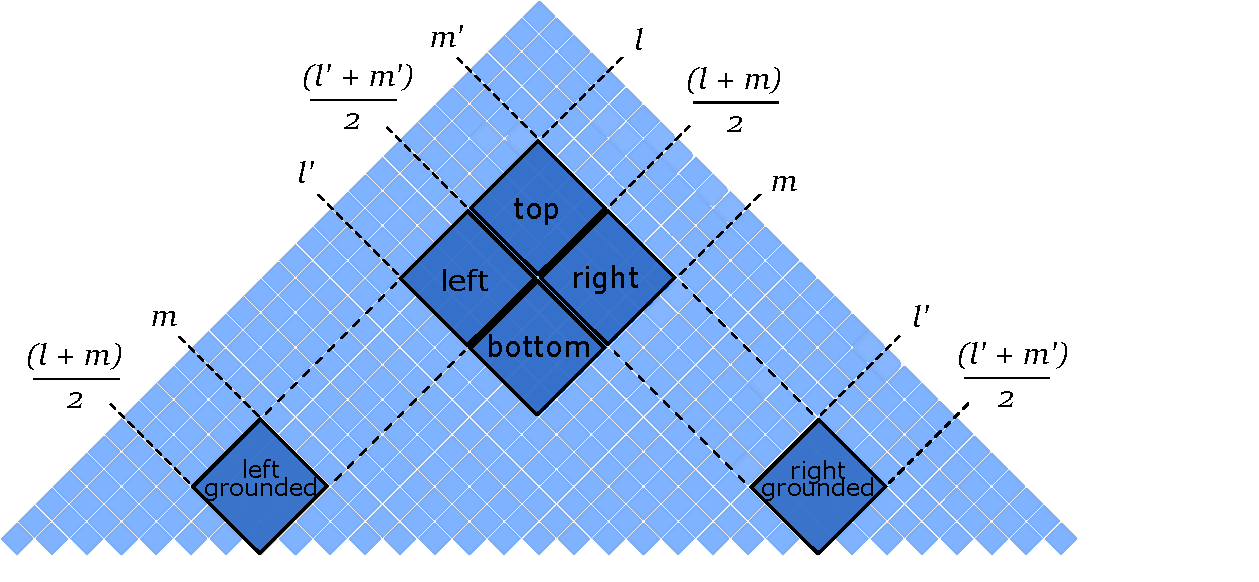
\includegraphics[width=200pt]{splitting_with_grounded2.pdf}
\centering
\caption{Matrix partition used in $complete(l, m, l', m')$ procedure} \label{fig1}
\end{figure}

Then Valiant described that product of multiplying of two submatrices of parsing table T can be provided as $|N|^2$ Boolean matrices (for each pair of nonterminals). Denote matrix corresponding to pair $(B, C) \in N \times N$ as $Z^{(B, C)}$, then $Z_{i, j}^{(B, C)} = 1$ if and only if $(B, C) \in Z_{i, j}$. It should also be noted that $Z^{(B, C)} = X^{B} \times Y^{C}$. So, matrix multiplication in \textbf{Definition 4} can be replaced by Boolean matrix multiplication, each of which can be computed independently. Following these changes, time complexity of \textbf{Algorithm 1} is $O(|G|BMM(n)log(n))$ for an input string of length n, where BMM(n) is the number of operations needed to multiply two Boolean matrices of size $n \times n$.

\section{Modification of Valiant's algorithm}
 
In this section we describe the modification of Valiant's algorithm, which has a number of advantages, such as possibility to broke it down into several subtasks that can be processed independently. Also this version can be simply applied to the string-matching problem, which often arises in text editing, DNA and RNA sequence analysis.

\subsection{New approach}
 
The main change of this modification is the possibility to divide the parsing table into layers of disjoint submatrices of the same size. The division we have made from the reorganization of the matrix multiplication order is presented in \textbf{Figure 2}.  The layers are computed successively from the bottom up.

\begin{figure}[h]

\includegraphics[width=250pt]{layers2.eps}
\centering
\caption{Matrix partition on V-shaped layers.} \label{fig1}
\end{figure}

Let us consider the pseudo-code of the modification, which is written in \textbf{Algorithm 2}. The procedure $main()$ computes the lowest layer ($T_{l, l+1}$), and then divide the table into layers, described earlier, and computes them through the $completeVLayer()$ call. Thus, $main()$ computes all elements of parsing table T correctly.

For the sake of brevity, we introduce $left(m), right(m), top(m), bottom(m),$ $rightgrounded(m)$ and $leftgrounded(m)$ functions which returns the nessesary submatrix for matrix $m = (l, m, l', m')$ according to \textbf{Figure 1}.

Denote some subsidiary functions for matrix layer $M$:
 \begin{itemize}
  \item $bottomsublayer(M) = \{bottom(m) | m \in M \}$,
  \item $lrsublayer(M) = \{left(m) | m \in M \} \cup \{right(m) | m \in M \}$,
  \item $topsublayer(M) = \{top(m) | m \in M \}$.
\end{itemize}
 
The procedure $completeVLayer(M)$ takes an array of disjoint submatrices M. For each $m = (l, m, l', m') \in M$ this procedure computes $left(m)$, $right(m)$, $top(m)$. The procedure assumes that the elements of $bottom(m)$ and all $T_{i, j} \forall l \leq i < j < m,  l' \leq i < j < m'$ are already constructed. Also it is assumed that the current value of  $P[i, j] =  \{ (B, C) |\exists (m \le k < l'): a_{i + 1}...a_{k} \in L(B), a_{k + 1}...a_{j} \in L(C)\}$ $\forall l \leq i < m,  l' \leq j < m'$.
 
The procedure $completeLayer(M)$ also takes an array of disjoint submatrices M, but unlike the previous one, it computes $T_{i, j} \forall (i, j) \in m$. This procedure, just as in the previous case, assumes that  $T_{i, j} \forall l \leq i < j < m,  l' \leq i < j < m'$ are already constructed and the current value of  $P[i, j] =  \{ (B, C) |\exists (m \le k < l'): a_{i + 1}...a_{k} \in L(B), a_{k + 1}...a_{j} \in L(C)\}$ $\forall l \leq i < m,  l' \leq j < m'$.

% Algorithm2
\begin{algorithm}
\SetAlgoNoLine
\KwIn{Grammar $G = (\Sigma, N, R, S), w = a_{1}...a_{n}, n \geq 1, a_{i} \in \Sigma$, where  n + 1 --- power of two}
\underline{main()}{:}{
 
 \For {$l \in \{1, \ldots, n \}$}{$T_{l, l + 1} = \{A | A \rightarrow a_{l + 1} \in R\}$}
 \For{$1 \le i < k $}{
 layer = $\textit{constructLayer(i)}$\;
 \textit{completeVLayer(layer)}
 }
 \BlankLine
 }
 
\underline{constructLayer(i)}{:}{
 \BlankLine
 $\{B | \exists k \geq 0 : B = (k*2^i, (k+1)*2^i, (k + 1)*2^i, (k+2)*2^i) \}$
 \BlankLine
    }
\underline{completeLayer(M)}{:}{
\BlankLine
\If {$\forall (l, m, l', m') \in M \quad (m - l = 1)$}{\For{$ (l, m, l', m') \in M$}{$T_{l, l'} = f(P_{l, l'})$\;}}
\Else{
\textit{completeLayer(bottomsublayer(M))}\;
\textit{completeVLayer(M)}
}
\BlankLine
}
 
\underline{comleteVLayer(M)}{:}{
 \BlankLine
 multiplicationTask1 = $\{left(subm), leftgrounded(subm), bottom(subm) | subm \in M \} \cup \linebreak  \{right(subm), bottom(subm), rightgrounded(subm) | subm \in M\}$\;
 \BlankLine
 multiplicationTask2 = $\{top(subm), leftgrounded(subm), right(subm) | subm \in M\}$\;
 \BlankLine 
 multiplicationTask3 = $\{top(subm), left(subm), rightgrounded |subm \in M\}$\;
 \BlankLine
 \textit{performMultiplications(multiplicationTask1)}\;
 \textit{completeLayer(lrsublayer(M))}\;
 \textit{performMultiplications(multiplicationTask2)}\;
 \textit{performMultiplications(multiplicationTask3)}\;
 \textit{completeLayer(topsublayer(M))}
 
 }

\caption{Parsing by matrix multiplication: Modified Version}
\end{algorithm}
 
\textbf{Algorithm 3} describes how the procedure $performMultiplication(task)$, where $task$ is an array of a triple of submatrices, works. It is worth mentioning that, as distinct from the original algorithm, $|tasks| \ge 1$ and all these multiplications can be computed independently.


 % Algorithm3
\begin{algorithm}[h!]
\SetAlgoNoLine
\underline{performMultiplication(task)}{:}{\\
\For{$ (m, m1, m2) \in M$}{$P_{m} = P_{m} \cup (T_{m1} \times T_{m2})$\;}
}
\caption{}
\end{algorithm}

\subsection{Proof of correctness}

We provide the proof of correctness and time complexity for the proposed modification in this section. 

\begin{theorem}
Let M be a submatrix array. Assume that $T[i, j] =  \{ A |  a_{i + 1}...a_{j} \in L(A)\}$ $\forall l \leq i < j < m,  l' \leq i < j < m'$ and $P[i, j] =  \{ (B, C) |\exists (m \le k < l'): a_{i + 1}...a_{k} \in L(B), a_{k + 1}...a_{j} \in L(C)\}$ $\forall l \leq i < m,  l' \leq j < m'$ $\forall (l, m, l', m') \in M$.

Then the procedure $\textit{completeLayer(M)}$, returns correctly computed sets of $T[i, j]$ $\forall l \leq i \le m,  l' \leq j \le m'$ $\forall (l, m, l', m') \in M$. 
\end{theorem}
%
% the environments 'definition', 'lemma', 'proposition', 'corollary',
% 'remark', and 'example' are defined in the LLNCS documentclass as well.
%
\begin{proof}
Induction on $\textit{m - l}$. (Hereinafter denoting (l, m, l', m') as a typical example of array M, and all the computations are implemented for all submatrices in M).

The base case: $\textit{m - l}$ = 1. There is only one element to compute, and $P[l, l'] =  \{ (B, C) |  a_{l + 1}...a_{l'} \in L(B)L(C)\}$. Further, algorithm computes $f(P[l, l'])$ = \linebreak $\{ A |  a_{l + 1}...a_{l'} \in L(A)\}$, so $T[l, l']$ computed correctly.

For the induction step, assume that (l1, m1, l2, m2) is correctly computed for $m2 - l2 = m1 - l1 > m - l$.

Let us consider complete $\textit{completeLayer(M)}$, where $\textit{m - l} >$ 1.

Firstly, consider $\textit{completeLayer(bottom = \{$(\frac{l+m}{2}, m, l', \frac{l'+m'}{2})$\})}$, as theorem conditions are fulfilled, then this call returns correct sets $T[i, j]$ $\forall (i, j) \in bottom$ (hereinafter is means $\forall (i, j) \in m$ $\forall m \in bottom$). All submatrices with size \linebreak $m1 - l1 > m - l$, all previous layers and also $\textit{bottom(M)}$ are correct, \linebreak so,  $\textit{completeVLayer(M)}$ can be called, and $\textit{multiplicationByTask(task1)}$ adds to each $P[i, j]$ $\forall (i, j) \in left = \{(\frac{l+m}{2}, m, l', \frac{l'+m'}{2}))\}$ all pairs $\{(B, C) |\exists (\frac{l+m}{2} \le k < l'): a_{i + 1}...a_{k} \in L(B), a_{k + 1}...a_{j} \in L(C)\}$ and $\forall (i, j) \in right = \{(\frac{l+m}{2}, m, \frac{l'+m'}{2}, m')\}$ all pairs $\{ (B, C) |\exists (m \le k < \frac{l'+m'}{2}): a_{i + 1}...a_{k} \in L(B), a_{k + 1}...a_{j} \in L(C)\}$. Now all the theorem conditions are fulfilled so, it is possible to call \linebreak $\textit{completeLayer($left \cup right$)}$, which returns correct sets $T[i, j]$ $\forall (i, j) \in ($left \cup right$)$. 

Next, \textit{multiplicationByTask(task2)} and \textit{multiplicationByTask(task3)} add to each $P[i, j]$ $\forall (i, j) \in top = \{(l, \frac{l+m}{2}, \frac{l'+m'}{2}, m'))\}$ all pairs $\{(B, C) |\exists (\frac{l+m}{2} \le k < m)$ and $(l' \le k < \frac{l'+m'}{2}) : a_{i + 1}...a_{k} \in L(B), a_{k + 1}...a_{j} \in L(C)\}$. Now all the theorem conditions are fulfilled so, it is possible to call $\textit{completeLayer(top)}$, which returns correct sets $T[i, j]$ $\forall (i, j) \in top$. 

Thus, all $T[i, j]$ $\forall (i, j) \in M$ are computed correctly.
\end{proof}

\begin{theorem}
Let M be a submatrix array. Assume that, $T[i, j] =  \{ A |  a_{i + 1}...a_{j} \in L(A)\}$ $\forall l \leq i < j < m,  l' \leq i < j < m'$ and $\forall b1 \leq i < b2$,  $b3 \leq j < b4$, where $(b1, b2, b3, b4) = (\frac{l+m}{2}, m, l', \frac{l'+m'}{2})$, also $P[i, j] =  \{ (B, C) |\exists (m \le k < l'): a_{i + 1}...a_{k} \in L(B), a_{k + 1}...a_{j} \in L(C)\}$ $\forall l \leq i < m,  l' \leq j < m'$ $\forall (l, m, l', m') \in M$.

Then, the procedure $\textit{completeVLayer(M)}$, returns correctly computed sets of $T[i, j]$ $\forall l \leq i \le m,  l' \leq j \le m'$ $\forall (l, m, l', m') \in M$. 
\end{theorem}

\begin{proof}
The proof is similar to the proof of Theorem 1.
\end{proof}

\begin{note}
Function $\textit{costructLayer(i)}$ returns $2^{k - i} - 1$ matrices of size $2^i$.
\end{note}

\begin{lemma}
\
\begin{itemize}
 \item $\forall i \in \{ 1, .., k - 1\}$  $\sum{|layer|}$ for the calls of \textit{completeVLayer(layer)} where $\forall (l, m, l', m') \in layer$ with $m - l = 2^{k - i}$  is exactly $2^{2i - 1} - 2^{i - 1}$;
 \item $\forall i \in \{ 1, .., k - 1\}$ products of submatrices of size $2^{k - i} \times 2^{k - i}$ are calculated exactly $2^{2i - 1} - 2^{i}$
\end{itemize}
\end{lemma}

\begin{proof}
The base case: i = 1. $\textit{completeVLayer(layer)}$ where $\forall (l, m, l', m') \in layer$ with $m - l = 2^{k - 1}$ is called only once in the  $\textit{main()}$ and $|layer| = 1$. So, $2^{2i - 1} - 2^{i - 1} = 2^1 - 2^0 = 1$.

For the induction step, assume that $\forall i \in \{ 1, .., j\}$ $\sum{|layer|}$ for the calls of $\textit{completeVLayer(layer)}$ where $\forall (l, m, l', m') \in layer$ with $m - l = 2^{k - i}$  which is exactly $2^{2i - 1} - 2^{i - 1}$.

Let us consider i = j + 1. 

Firstly, it is the call of \textit{completeVLayer(costructLayer(k - i))}, where \textit{costructLayer(i)} returns $2^i - 1$ matrices of size $2^i$. Secondly, \textit{completeVLayer(layer)} is called 3 times for the left, right and top submatrices of size $2^{k - (i - 1)}$. Finally, \textit{completeVLayer(layer)} is called 4 times for the bottom, left, right and top submatrices of size $2^{k - (i - 2)}$, except $2^{i - 2} - 1$ matrices which were already computed.

Then, $\sum{|layer|} = 2^{i} - 1 + 3 \times (2^{2(i - 1) - 1} - 2^{(i - 1) - 1}) + 4 \times (2^{2(i - 2) - 1} - 2^{(i - 2) - 1}) - (2^{i - 2} - 1) = 2^{2i - 1} - 2^{i - 1}$. 

To calculate the number of products of submatrices of size $2^{k - i} \times 2^{k - i}$, we consider the calls of \textit{completeVLayer(layer)} where $\forall (l, m, l', m') \in layer$ with $m - l = 2^{k - (i - 1)}$, which is $2^{2(i - 1) - 1} - 2^{(i - 1) - 1}$. During these calls \textit{performMultiplications} run 3 times, $|multiplicationTask1| = 2 \times 2^{2(i - 1) - 1} - 2^{(i - 1) - 1}$ and \linebreak $|multiplicationTask2|$ = $|multiplicationTask3| = 2^{2(i - 1) - 1} - 2^{(i - 1) - 1}$. So, the number of products of submatrices of size $2^{k - i} \times 2^{k - i}$ is $4 \times (2^{2(i - 1) - 1} - 2^{(i - 1) - 1}) = 2^{2i - 1} - 2^{i}$.
\end{proof}

\begin{theorem}
The time complexity of the Algorithm 1 is $O(|G|BMM(n)log(n))$ for an input string of length n, where G is a context-free grammar in Chomsky normal form, BMM(n) is the number of operations needed to multiply two Boolean matrices of size $n \times n$.
\end{theorem}

\begin{proof}
The proof is almost identical with that of the theorem given by Okhotin~\cite{okhotin}, because, as shown in the last lemma, the Algorithm 1 has the same number of products of submatrices.
\end{proof}

To summarize, the correctness of the modification was proved and it was shown that the time complexity remained the same as in Valiant's version.

\subsection{Algorithm for substrings}

Next we show how our modification can be applied to the problem hat  arose  at  the  intersection  of  the  theory  of  formal  languages and bioinformatics -- the string-matching problem.

So if we want to find all substrings of size s which can be derived from a start symbol for an input string of size $n = 2^k$, we need to compute layers with submatrices of size $\le 2^{l'}$, where $ 2^{l' - 2} < s \le 2^{l' - 1}$.

$l' = k - (m - 2)$, $(m - 2) = k - l'$

$ C \sum\limits_{i=m}^k 2^{2i - 1} \cdot 2^{\omega(k - i)} \cdot f(2^{k - i}) = C \cdot 2^{\omega l'}\sum\limits_{i=2}^{l'} 2^{(2 - \omega)i} \cdot 2^{2(k - l') - 1} \cdot f(2^{l' - i}) \le C \cdot 2^{\omega l'} f(2^{l'}) \cdot 2^{2(k - l') - 1} \sum\limits_{i=2}^{l'} 2^{(2 - \omega)i} = BMM(2^{l'}) \cdot 2^{2(k - l') - 1} \sum\limits_{i=2}^{l'} 2^{(2 - \omega)i}$ 

Thus, time complexity for searching all substrings is  $O(|G|BMM(2^{l'})(l' - 1))$, while time complexity for the full input string is $O(|G|BMM(2^k)(k - 1))$. In contract to the modification, Valiant's algorithm completely calculate at least 2 triangle submatrices of size $\frac{n}{2}$, which mean minimum asymptotic complexity  $O(|G|BMM(2^{k - 1})(k - 2))$. Make a conclusion that the modification is asymptotically faster for substrings of size s $<<$ n  than the original algorithm. 

\section{Evaluation}

After demonstrating the theoretical value of the proposed solution, the next step of our work was to show its applicability on real data. Both algorithms (original Valiant's version and the modification) were compared on context-free grammar G  ...?picture?...  which is used to approximate the secondary structure of the biological sequences. As it was mentioned before, the secondary structure is a very powerful instrument for species classification and identification problem. Parsing algorithms based on matrix multiplication helps efficiently find subsequences with features specific to the secondary structure.

The algorithms were implemented using a library for fast Boolean matrix multiplication M4RI~\cite{m4ri}. The biological sequences were taken from this dataset[]. 

All tests were run on a PC with the following characteristics:
\begin{itemize}
\item OS:
\item CPU:
\item System Type:
\item RAM:
\end{itemize}

The results of experiments which are presented ?...? show that our modification can be efficiently applied to the string matching problem as it demonstrates good time on real data. 


\section{Conclusion and Future Work}

The main goal of this work was to find an effective solution for the string-matching problem that arose at the intersection of the theory of formal languages and bioinformatics. We proposed a modification of Valiant's algorithm partially dealing with this problem. Also we proved its applicability by showing the asymptotic complexity concerning substring searching. 



%
% ---- Bibliography ----
%
% BibTeX users should specify bibliography style 'splncs04'.
% References will then be sorted and formatted in the correct style.
%
% \bibliographystyle{splncs04}
% \bibliography{mybibliography}
%
\begin{thebibliography}{8}
\bibitem{chomsky1}
Chomsky, N.: On certain formal properties of grammars. Information and control \textbf{2}(2), 137--167 (1959)

\bibitem{chomsky2}
Chomsky, N. and Schützenberger M. P.: The algebraic theory of context-free languages. In: Studies in Logic and the Foundations of Mathematics vol. 35. pp. 118--161 Elsevier (1963)

\bibitem{rivas}
Rivas, E. and Eddy, S. R: The language of RNA: a formal grammar that includes pseudoknots. Bioinformatics \textbf{16}(4), 334–-340 (2000)

\bibitem{knudsen}
Knudsen, B. and Hein, J.: RNA secondary structure prediction using stochastic context-free grammars and evolutionary history. Bioinformatics (Oxford, England) \textbf{15}(6), 446–-454 (1999)

\bibitem{yuan}
Yuan, C. and Lei, J. and Cole, J. and Sun, Y.: Reconstructing 16S rRNA genes in metagenomic data. Bioinformatics \textbf{31}(12), i35–-i43 (2015)

\bibitem{dowell}
Dowell, R. D. and Eddy, S. R.: Evaluation of several lightweight stochastic context-free grammars for RNA secondary structure prediction. BMC bioinformatics \textbf{5}(1), 71 (2004)

\bibitem{bernardy}
Bernardy, J.P., Claessen K.: Efficient divide-and-conquer parsing of practical context-free languages. In: ACM SIGPLAN Notices, vol. 48. no. 9, pp. 111-122 ACM (2013)

\bibitem{kasami}
Kasami, T.: An efficient recognition and syntax-analysis algorithm for context-free languages. Coordinated Science Laboratory Report no. R-257 (1966)

\bibitem{younger}
Younger, D.H.: Recognition and parsing of context-free languages in time n3. Information and control \textbf{10}(2), 189--208 (1967)

\bibitem{earley}
Earley, J.: An efficient context-free parsing algorithm. Communications of the ACM \textbf{13}(2), 94--102 (1970)

\bibitem{valiant}
Valiant, L. G.: General context-free recognition in less than cubic time. Journal of computer and system sciences \textbf{10}(2), 308--315 (1975)

\bibitem{okhotin}
Okhotin, A.: Parsing by matrix multiplication generalized to Boolean grammars. Theoretical Computer Science \textbf{516}, 101--120 (2014)

\bibitem{m4ri}
The M4RI Library -- Version 20121224, \url{http://m4ri.sagemath.org}. Last accessed 5
Jan 2019


\end{thebibliography}
\end{document}
